\documentclass[11pt,a4paper]{article}
\usepackage[hyperref]{acl2020}
\usepackage{times}
\usepackage{latexsym}
\usepackage{graphicx}
\renewcommand{\UrlFont}{\ttfamily\small}

% This is not strictly necessary, and may be commented out,
% but it will improve the layout of the manuscript,
% and will typically save some space.
\usepackage{microtype}

\usepackage{amsmath,amssymb}
\DeclareRobustCommand{\bbone}{\text{\usefont{U}{bbold}{m}{n}1}}

\DeclareMathOperator{\EX}{\mathbb{E}}% expected value

\aclfinalcopy % Uncomment this line for the final submission
%\def\aclpaperid{***} %  Enter the acl Paper ID here

%\setlength\titlebox{5cm}
% You can expand the titlebox if you need extra space
% to show all the authors. Please do not make the titlebox
% smaller than 5cm (the original size); we will check this
% in the camera-ready version and ask you to change it back.

\newcommand\BibTeX{B\textsc{ib}\TeX}

\title{Linear-BERT: Data-Efficient Learner for Token Classification}

\author{Pin-Jie Lin\thanks{* Equal Contribution.}\ , Fabian Stiewitz\footnotemark[1] \\
  Department of Language Science and Technology \\
  Saarland University \\
  \texttt{\{pili00001, s8fastie\}@stud.uni-saarland.de}}


% \author{Pin-Jie Lin\thanks{* Equal Contribution.} \\
%   Saarland University \\
%   Dept. of Language Science and Technology \\
%   \texttt{pili00001@} \\\And
%   Fabian Stiewitz\footnotemark[1] \\
%   Saarland University \\
%   Dept. of Language Science and Technology \\
%   \texttt{s8fastie@} \\}

\date{}

\begin{document}
\maketitle
\begin{abstract}

The vast majority of tasks in NLP have achieved promising results by fine-tuning large-scale pre-trained models. However, fine-tuning the entire model carries high memory requirements and might be inefficient. In this work, we systematically evaluate the capacities of the contextual representations obtained from the BERT's layers. We demonstrate that it is unnecessary to add the classifier on top of BERT. Our Linear-BERTs trained on full datasets and small subsets achieve $0.96$ and $.95$ F1 scores respectively. The experiment shows that Linear-BERTs trained on small subsets have competitive results compared to the models trained on full datasets where the model uses less than 10\% of the full dataset.

\end{abstract}

\section{Introduction}

Current state-of-the-art representation learning algorithms are training the contextual representations to provide generalized and information-rich features for downstream tasks. The attempts to leverage the contextual representation can broadly be categorized into three approaches. They either fine-tune the entire model, insert the adapter module or simply add a classifier on the top of pre-trained models.

However, they generally require large amounts of data and computation to be effective. We are curious about how to apply a large pre-trained model to limited supervised data. This research aims to answer the two questions: Does fine-tuning BERT require large amounts of data to be effective? Meanwhile, should we train the classifier on top of the BERT's last layer? To answer these questions, we employ Linear-BERT to test the performances using full and a smaller subset of data. Furthermore, we evaluate the qualities of the representations obtained from different BERT's layers. 

As an alternative to previous works, we systematically evaluate the frozen BERT with one classifier head on different BERT's layers, Linear-BERT\footnote{source code available at: \url{https://github.com/pjlintw/Transformer-py}}. We are increasing the amount of layers to train both full and small subset of OntoNotes dataset.


\section{Linear-BERT}


In this section, we define the Linear-BERT as a token-level classifier where the pre-trained masked language model combines a linear classifier head on one of the encoder's layers.

Given an unlabeled dataset $X$ consisting of the sentence $x = (x_{1}, x_{2}, ...{x_n})$. The sequence of tokens will be tokenized into a corrupted sequence $\hat{x}$ with the mask token ${[MASK]}$. The BERT model predicts the missing token $\bar{x_{j}}$ at the position $j$ from a corrupted sentence without seeing it. The training objective for BERT is to reconstruct $\bar{x}$ from $\hat{x}$.

\begin{align*}
    L_{BERT}(x, \theta) = \EX(\sum_{j} - \log p_{\theta}(\bar{x_{j}}| \hat{x}))
\end{align*}


The Linear-BERT for token classification takes an input sequence of discrete tokens ${x}$ and produces a $d$-dimensional representation for each position. We denote a embedding $h_{i}^{l}$ as the embedding for the position {i} obtained from the $l$ layer. These contextual representations can be written as:

\begin{align*}
    h_{i}^{l} &= BERT^{l}(x) 
\end{align*}

where $2 \leq l \leq L$. The classifier layer uses the contextual representations from the second layer all the way down to layer $L$. We apply dropout and learn a projection from the hidden states to class logits, where we use them to minimize a cross entropy loss L for token classification.


\begin{align*}
    a_{i}^{l} &=  dropout(h_{i}^{1}) \\
    \hat{y_{i}} &= linear(a_{i}^{l}) \\
    L_{i} &= CrossEntropy(y_{i}, \hat{y_{i}}) \\
\end{align*}


\section{Experiment}

In all the experiments, we focus on sequence labelling tasks, OntoNotes and the feature-based approach with BERT, thus we freeze BERT's weights and only train the classifier.

\subsection{Experimental setup}

\paragraph{OntoNotes} We use the OntoNotes 4.0 dataset. It consists of 69880 examples with 49 POS tags. For the full and the small dataset,
we leverage two dataset sizes for the Linear-BERT training. We select 65880 as our full dataset and select 5760 examples
for the small subset of the data where the small dataset is less than 10\% of the full dataset. Both training sets use another 300 examples for the evaluation set and test set. This is to make sure that the Linear-BERTs are evaluated on the same criteria.

\paragraph{Architecture}

Linear-BERT is an architecture for evaluating the quality of extracted features from BERT. It is a pre-trained BERT model with a dropout layer and linear classifier. We use the pre-trained BERT with 12 layers and 110M parameters as the base model. Our approach is to train a classifier by adding a linear classification head on top of BERT's layers. In our experiment, we train multiple models with the classification head at different layers, from 2nd to the 12th layer. 

For the training Linear-BERT on the full dataset, we run 3 epochs on the full dataset. For the models on the small subset, we only use 5760 examples for training 120 steps. 


\paragraph{Hyperparameters}
For the BERT configuration, we follow mostly the original settings. The dimension of the BERT's hidden states is 768. The linear classifier projects 768 into a number of tags. We use 48 examples per batch size and set 42 as the seed for all experiments. The dropout rate is 0.1. We use $\beta_{1} = 0.99 $ and $\beta_{2} = 0.999 $ for AdamW optimizer. We tried  1e-2, 1e-3, 1e4, and 1e-5 learning rates. Only 1e-2 converges faster than others. We use 1e-2 for all the experiments. 

Furthermore, training the examples with padding to the maximal sequence length is extremely slow. We found 99\% percentile of sequence length is 63. Thus, we pad the input sequence to 63 and gain faster execution for training the networks. On average, training a Linear-BERT model on a small subset takes only around 20 minutes on an Intel i5 CPU. Training on the full dataset takes around 20 minutes on a Radeon RX 580 GPU.


\begin{figure}
\begin{center}
  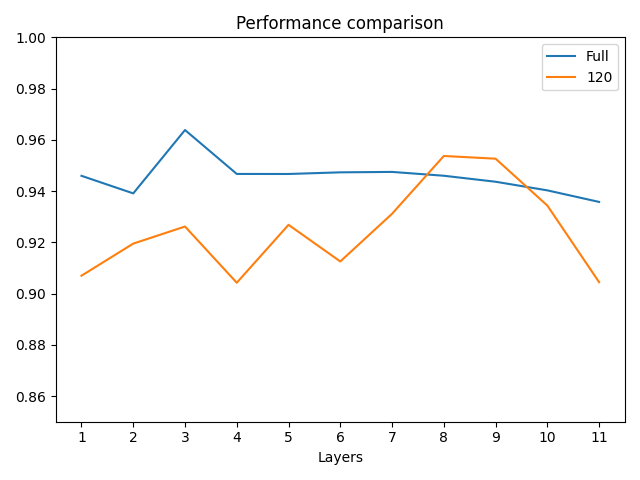
\includegraphics[width=\linewidth]{f1-comp.png}
  % f1-full.png: 640x480 px, 72dpi, 22.58x16.93 cm, bb=0 0 640 480
  \caption{\label{fig:f1-comp}The quality of contextual representations depends on the layer from which we extract features. Linear-BERT achieves the best 96 F1-score with a full dataset. The models using small amounts of training examples are competitive and slightly outperform in the 9th and 10th layers.
}
\end{center}
\end{figure}

\begin{figure}
\begin{center}
  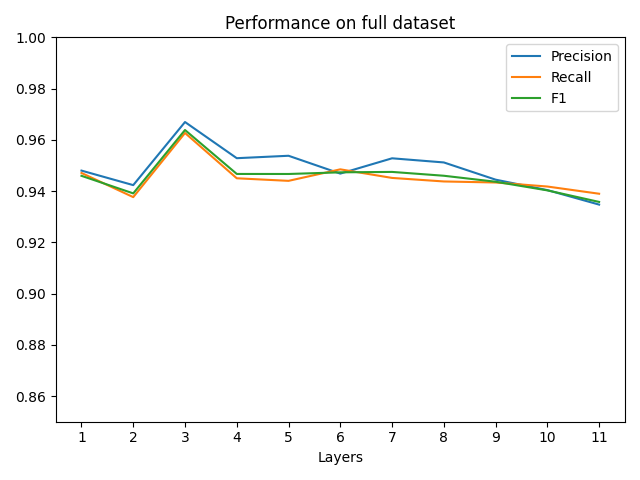
\includegraphics[width=\linewidth]{f1-full.png}
  % f1-full.png: 640x480 px, 72dpi, 22.58x16.93 cm, bb=0 0 640 480
  \caption{\label{fig:f1-full}The figure shows the precision, recall and F1-score for Linear-BERT on the full dataset. The Linear-BERT in 4th layer achieves 96 F1 score which is the best score among our experiment.}
\end{center}
\end{figure}

\subsection{Results}

We first compare the performance between the Linear-BERTs trained on the full dataset and a small subset, then provide more details on the capacities of Linear-BERT depending on the size of training examples.

\paragraph{Full and small datasets}
As shown in Figure~\ref{fig:f1-comp}, the quality of contextual representations depends on the layer from which we extract features. The figure shows the comparison of Linear-BERT trained on a full dataset and a small subset.  The best representation for a full dataset lie in the 4th layer. Linear-BERT trained on a small subset achieves the best F1 score in the 9th and 10th layer. Surprisingly, the Linear-BERT trained on a subset from the 9th and 10th layer are slightly better than fine-tuning on all the training examples. However, training the 11th layer and the last layer with 120 steps along drops quickly. The models trained on the whole dataset still outperform the models using a small amount of examples.

\paragraph{Linear-BERT on full dataset}
For the Linear-BERT on full dataset, we demonstrate that such models perform very small differences among the precision, recall and F1-scores at the final steps, as shown in Figure~\ref{fig:f1-full}. They are smooth across the layers.


\paragraph{Linear-BERT on small dataset}
In contrast, using a subset to fine-tune the classifier leads to rugged performance across layers. The best features show in the 9th and 10th layer. The F1-scores drop dramatically if we use the last two layers. On average, these models reach around $0.90$ F1 scores.
We demonstrate that Linear-BERT is a quick learner.


\section{Discussion}
Layers 9 and 10 for Linear-BERTs with limited update steps converge fast and slightly outperform the models trained on the full dataset. It is very possible that the features among BERT's layers have different capacities to converge. Therefore, Linear-BERT on a small dataset is less consistent and rugged.

In contrast, Linear-BERT achieves no significant difference in F1 score, along with more training examples. The contextual representations in the pre-trained model are powerful enough to transfer them to an unseen domain, so long as the number training examples is sufficient. If one has a sufficiently sized dataset to train their classifier, choosing every layer except for the 4th layer would acquire similar performance. On the other hand, with smaller training examples, the final results you could get are more rugged and they have obvious differences.

 
\begin{figure}
\begin{center}
  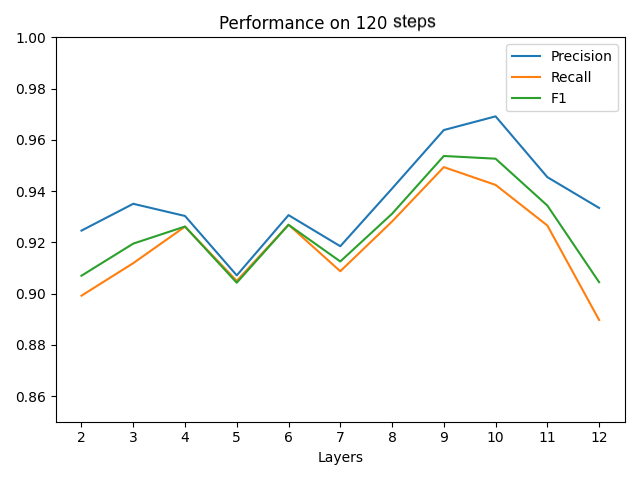
\includegraphics[width=\linewidth]{f1-120.png}
  % f1-full.png: 640x480 px, 72dpi, 22.58x16.93 cm, bb=0 0 640 480
  \caption{\label{fig:f1-120}Linear-BERTs trained on 120 steps are less consistent. The best representation for the small subset lies in the 9th and 10th layer. However, the last two layers drop quickly.}
\end{center}
\end{figure}

Finally, the last layer doesn't guarantee the best result. It performs the worst F1 score for the model trained on the full dataset. To our knowledge, the features extracted from the last layer is task-specific. They are used to predict the missing token from the corrupted sentence. Therefore, such contextual representations may not help to fully understand syntactic information.

\section{Conclusion}

In this paper we systematically evaluate the hidden states within the pre-trained transformer encoder that are better for syntactical classification tasks than the final layer. We suggest that it is unnecessary to train a classifier on top of BERT. For the small dataset, the Linear-BERTs are less consistent but still fairly performant. Most importantly, these models only use less than 1/10 of the entire dataset. The results demonstrate that training on 9th and 10th with few examples along could outperform models trained on full datasets. Our results demonstrate that a Linear-BERT on a small dataset is a data-efficient learner for token classification.

\end{document}
